\documentclass[12pt, a4paper]{book}
\usepackage[utf8]{inputenc}
\usepackage[croatian]{babel}
\usepackage[margin=1in]{geometry}
\usepackage{amsmath}
\usepackage{diplomski}
\usepackage{amssymb}
\usepackage{amsthm} 
\usepackage{mathtools}
\usepackage{hyperref}
\usepackage{graphicx}
\usepackage{multirow}
\usepackage{fancyhdr} % prored, numeriranje stranice...
\usepackage{amsfonts}
\usepackage{setspace}% za postavljanje praznina
\usepackage{color}
\usepackage{wasysym}
\usepackage{bbm}
\usepackage{multicol}
\usepackage{url}
\DeclareMathOperator {\sg}{sg}
\fancyhf{}
\renewcommand{\headrulewidth}{0pt}
\rfoot{\thepage}
\usepackage{paralist}
\usepackage{color}
\usepackage{tikz}
\usetikzlibrary{arrows,positioning,automata}
\PassOptionsToPackage{usenames,dvipsnames,svgnames}{xcolor}
 \newcommand{\HRule}{\rule{\linewidth}{0.5mm}}
\setlength\parindent{24pt}



\begin{document}
\renewcommand{\bibname}{Literatura}%ne želim da mi piše bibliografija već literatura
\begin{titlepage}
\begin{center}
\newtheorem{thm}{Teorem}[chapter] %u svakom poglavlju teoremi se numeriraju zasebno
%\theoremstyle{definition}
\newtheorem{defn}[thm]{Definicija} %enumeracija definicija jednaka enum teorem
\newtheorem{exa}[thm]{Primjer} % analogno s primjerima
\newtheorem{nap}[thm]{Napomena} % analogno s naomenom
\newtheorem{conj}[thm]{Slutnja} % analogno s slutnjom

\LARGE Sveučilište u Zagrebu \\[1cm] Prirodoslovno - matematički fakultet \\[1cm] Matematički odsjek\\[3cm]

\Large Seminar iz kolegija "Složenost algoritama" \\[0.5cm]

% Title
\HRule \\[0.4cm]
{ \huge \bfseries Složenost algoritama \\ Liptonov teorem}\\[0.4cm]

\HRule \\[4.4cm]

% Autor i mentor -> postavljanje ovoga na dno stranice...
\begin{minipage}{0.4\textwidth}
\begin{flushleft} \large
\emph{Student:\\}
Antonio Kovačić
\end{flushleft}
\end{minipage}
\begin{minipage}{0.4\textwidth}
\begin{flushright} \large
\emph{Mentor:\\}
Prof. dr. sc.\\ Mladen Vuković
\end{flushright}
\end{minipage}
\\[1cm]

\vfill 

% Bottom of the page
{\large Zagreb, 19. lipnja 2014.}

\end{center}
\end{titlepage}

\pagestyle{plain} % No headers, just page numbers
\pagenumbering{roman} % Roman numerals
\setcounter{page}{1}
\begingroup
\let\cleardoublepage\relax
\tableofcontents

\newpage


\begin{spacing}{1.5}
\setcounter{chapter}{1}
\begin{intro}
    \indent Premda su računala od svog postanka jako napredovala, a broj instrukcija koje se mogu obavljati u sekundi neprestano rastao, kroz posljednje desetljeće broj instrukcija u sekundi koje neko računalo može obaviti ne povećava se značajno. Ta činjenica zapravo i nije toliko začuđujuća, naime u uporabi je takozvani silicijski mikroprocesorski čip koji radi pregrijavanja i taljenja pri visokim temperaturama ne može ispuniti zahtjeve koje definiraju znanstvenici, inženjeri i programeri. U tu svrhu, počelo se sa proizvodnjom takozvanih višejezgrenih procesora radi ubrzanog obavljanja instrukcija - to jest paralelnog obavljanja nekog zadatka. Premda je i ta tehnološka inovacija doprinjela brzini rada računala, ona još uvijek ne može ispuniti zahtjeve koji se stavljaju pred nju.\\
    \indent Znanstvenici i inženjeri su u tu svrhu išli tražiti novo rješenje koje bi pomoglo pri nadilaženju tih zahtjeva. Jedno od njih je bilo upotreba istih tehnologija, ali različitog materijala, tako su na primjer rađeni eksperimenti gdje se kao materijal za izgradnju mikroprocesorskih čipova koristio galij arsenid, ali to se rješenje nije pokazalo dovoljno povoljno.\\
    \indent Kao alternativu, znanstvenici su pružali neke nove modele računala koji bi mogli udovoljit zahtjevima koji se pred njih stavljaju - to su, na primjer, DNA strojevi i kvantna računala. Sama struktura DNA i kapacitet memorije koji može pohraniti u sebe, dala je znanstvenicima novi model za izračunavanje: DNA izračunavanje. Osnovna ideja DNA izračunavanja je uporaba takozvanih dušićnih baza - adenina (A), gvanina (G), timina (T) i citozina (C) te konstruiranje instrukcija koje su analogne mikrobiološkim i biokemijskim procesima vezanim za DNA lance. Ovim radom proširujemo pojam DNA izračunljivosti te analiziramo detaljnije složenost DNA računala, odnosno jedan od centralnih teorema o složenosti DNA računala - a to je Liptonov teorem. U kasnijem dijelu rada ćemo predstaviti mane i prednosti DNA računala. 
\end{intro}
\newpage
\section{DNA izračunljivost}
\label{sec:DNAizr}
DNA stroj, kao ni DNA izračunavanje nećemo striktno definirati već će definicija biti opisna - u definiciji ćemo reći koje operacije DNA stroj može izvršavati, i što pri tome mora biti zadovoljeno.\\ Prije nego definiramo DNA stroj moramo definirati neke pojmove iz logike sudova i kombinatorike.
\begin{defn}
\textbf{Alfabet} je proizvoljan konačan skup, čije elemente nazivamo \textbf{simboli}.\\
Neka je $n \in \mathbb{N}$ proizvoljan te $A$ proizvoljan alfabet, proizvoljni element $w \in A^n$ zovemo \textbf{riječ alfabeta A}. Neka su $s_1,..., s_n \in A$, riječ $w=(s_1,...,s_n)$ alfabeta A još zapisujemo kao $w=s_1s_2...s_n$. Smatramo da postoji riječ alfabeta A, koju ćemo označavati s $\varepsilon$, koja se ne sastoji ni od jednog simbola i zovemo je \textbf{prazna riječ}. Po dogovoru smatramo da je $A^0=\{\varepsilon\}$. Skup svih riječi alfabeta $A$ označavamo sa $A^*$. Neka su $a=a_1...a_m$, te, $b=b_1...b_k \in A^*$, kažemo da je riječ $c \in A^*$ nastala \textbf{konkatenacijom} riječi $a$ i $b$ ako vrijedi $c=ab=a_1...a_mb_1...b_k$. Kažemo da je riječ $c \in A^*$ podriječ riječi $a \in A^*$, ako postoje riječi $b, d \in A^*$ tako da je $a=bcd$. \textbf{Duljina riječi} se definira kao funkcija $d:A^*\to \mathbb{N}$ sa:
\begin{align*}
	d(\varepsilon) :&= 0 \\
	d(wa) :&= d(w)+1, \quad a \in A
\end{align*}
\end{defn}
\begin{defn}
Neka je S proizvoljan konačan skup, a $m:S \to \mathbb{N}$ proizvoljna funkcija. \textbf{Multiskup M na skupu S} je uređeni par $M=(S,m)$. Za proizvoljan $x\in S$, $m(x)$ zovemo \textbf{kratnost} od $x$. \textbf{Kardinalnost multiskupa M} (broj elemenata), u oznaci $|M|$, se definira kao:
\[|M|:=\sum_{x \in S} m(x)\]
\end{defn}
\begin{defn}
 \textbf{DNA lanac} je proizvoljna riječ alfabeta \{A (adenin), G (gvanin), T(timin), C (citozin)\}. DNA stroj se sastoji od konstantnog broja konačnih skupova koje nazivamo \textbf{epruvete}, a čiji su elementi DNA lanci. Za proizvoljnu epruvetu K DNA stroja definiramo multiskup $MulS(K)$ kao multiskup svih riječi koje predstavljaju DNA lance sadržane u epruveti K. U DNA stroju su definirane slijedeće instrukcije:
    \begin{itemize}
        \item Kopiraj($K_1$,$K_2$) $\to$ uz pretpostavku da je $K_2$ = $\emptyset$ , kopira MulS($K_1$) u MulS($K_2$) time više $K_2$ nije prazan
        \item Spoji($K_1$, $K_2$, $K$) $\to$ uz pretpostavku da $K$=$\emptyset$: \[MulS(K)=MulS(K_1)\cup MulS(K_2) \]
        \item Uoči($K$) $\to$ ispituje je li $MulS(K)\neq\emptyset$, ako je rezultat operacije je $\top$, inače $\bot$. Također se može pročitati sadržaj epruvete $MulS(K)$.
        \item Odvoji(K,w) $\to$ za skup $K$ i riječ $w$ (iz $MulS(K)$) izbacuje sve riječi iz $K$ koje kao podriječ ne sadrže riječ $w$
        \item Izvadi(K,w) $\to$ $K\backslash Odvoji(K,w)\to $izbacuje sve riječi iz $K$ koje sadrže $w$
        \item Odvoji\textunderscore Pref(K,w) $\to$ izbacuje sve riječi iz K koje ne sadrže w kao prefiks
        \item Odvoji\textunderscore Suff(K,w) $\to$ izbacuje sve riječi iz K koje ne sadrže w kao sufiks
        \item Proširi(K) $\to$ multiskupu MulS(K) još jednom dodaje elemente od K
        \item Izdvoji\textunderscore po\textunderscore duljini(K, l) $\to$ iz K izbacuje sve riječi čija je duljina različita od l
        \item Konkatenacija(K) $\to$ na slučajan način izvodi operaciju konkatenacije nad riječima iz MulS(K) tako da duljina novonastalih riječi ne bude veća od neke konstante, a vraća multiskup koji sadrži sve riječi nastale tom konkatenacijom. Vjerojatnost nastajanja duljih riječi je veća. Ukoliko MulS(K) prije izvođenja ove operacije nad epruvetom K sadrži veliki broj kopija svake od riječi, tada će MulS(K) nakon izvođenja ove operacije nad epruvetom K sadržavati sve moguće kombinacije elemenata iz K.
            \begin{itemize}
                \item \textbf{Biološki komplement} DNA lanca H definiramo kao DNA lanac koja ima jednako znakova kao i H, ali je svaki znak A zamijenjen znakom T, a svaki znak C znakom G i obratno, i označavamo je s $\overline{H}$
                \item Neka riječ H ima duljinu $n \in 2\mathbb{N}$, tada definiramo \textbf{biološki prefiks} riječi H kao biološki komplement riječi sastavljene od prvih $\frac{n}{2}$ znakova iz H, slično definiramo i \textbf{biološki sufiks} riječi H kao biološki komplement riječi sastavljene od zadnjih $\frac{n}{2}$ znakova riječi H
                \item Smatramo da je operacija konkatenacije nad riječima H i J dopuštena ako postoji riječ L takva da je biološki sufiks od H prvih $\frac{n}{2}$  znakova od L, a biološki prefiks od J prvih $\frac{n}{2}$ znakova od L
            \end{itemize}
    \item Izreži(K) $\to$ na slučajan način “skraćuje” riječi iz MulS(K) do neke fiksne duljine
    \item Izaberi(K) $\to$ na slučajan način iz MulS(K) izabire neku riječ te “generira” novi skup sastavljen od samo te riječi

    \end{itemize}
    \textbf{Program za DNA stroj} definiramo kao konačan niz gornje navedenih instrukcija. U svakom koraku programa se može izvesti točno jedna instrukcija.  Kažemo da program P za DNA stroj \textbf{izračunava} funkciju $f:S \subseteq \mathbb{N}^k \to \mathbb{N}$ ako vrijedi:\\
$\vec{x}=(x_1,...,x_k) \in S$ ako i samo ako program P za DNA stroj s ulazom  $\vec{x}$ (reprezentiranim pomoću DNA lanaca) u epruveti K završi s izvršavanjem te na kraju izvršavanja vrijedi \textit{Uoči(K)}$=\top$ te je pri tome $K=\{f(\vec{x})\}$.\\
Kažemo da je funkcija $f: S\subset \mathbb{N}^k \to \mathbb{N}$ \textbf{DNA izračunljiva} ako postoji program za DNA stroj koji ju izračunava.
\end{defn}
\begin{nap}
Vidimo da se sve ove operacije izvršavaju nad jednom epruvetom u jednom koraku, odnosno multiskupom $MulS(K)$. Što je veća kardinalnost multiskupa $MulS(K)$, to se više operacija na riječima izvrši istovremeno, a u stvarnom svijetu sve te operacije imaju svoje "biokemijske analogone" - biokemijske reakcije. Takvo računalo zapravo možemo interpretirati kao superračunalo s izuzetno velikim brojem procesora. U pozadini svega toga se zapravo krije masivni paralelizam. Memoriju DNA računala zapravo predstavljaju epruvete. Jasno je odakle naziv epruvete.\\
Uočimo da je $MulS(K)$ definiran nad konačnim skupom pa je i on konačan - no vidimo da se on zapravo može proširiti nizom operacija \textit{Proširi} tako da je njegov kardinalitet izrazito velikog reda (nadeksponencijalnog) , ali u praksi se već sada zaključuje da to neće biti uvijek moguće - naime broj DNA lanaca u epruveti (laboratorijskoj) biti će ograničen volumenom te epruvete.\\
Uočimo da operacija konkatenacije uključuje vjerojatnosni efekt - \textit{vjerojatnost nastajanja duljih riječi konkatenacijom je veća} - odnosno dvije riječi iz skupa $K$ koje će se konkatenirati neće biti izabrane na slučajan način - već tako da se pokuša dobiti riječ maksimalne duljine (maksimalna duljina je određena nekom konstantom). Iz toga očito možemo vidjeti da sam ishod DNA računanja nije sasvim siguran  - no u praksi se pokazuje (pri sintezi DNA lanaca) da je to moguće - u tu svrhu je i uvedena pretpostavka da će  se, ukoliko $MulS(K)$ sadrži velik broj kopija od svake riječi iz $K$, dobiti svaka moguća konkatenacija riječi iz $K$.\\
Nadalje, u stvarnosti - se biokemijski gledano nakon operacije ekstrahiranja (Odvoji(K,w)) zapravo ne gube one riječi koje ne sadrže riječ kao podriječ, već se one riječi koje sadrže w kao podriječ stavljaju u drugu epruvetu (laboratorijsku), tako da se orginalna epruveta sa riječima koje ne sadrže riječ w kao podriječ i dalje može koristiti. Izvorno je model DNA računala tako i izgledao, a ovo je "modificirani" model DNA. Matematički koncept stvarne operacije Odvoji(K,w) bi bio ovakav zapravo:
\[T_1 \leftarrow Extract(K,w)\]
A sada bi za funkciju kratnosti $m_K$ vrijedilo $m_K(x)=0, \forall	x \in T_1$, gdje je $m_K$ pripadna funkcija kratnosti multiskupa $MulS(K)$. Upravo je taj izvorni koncept DNA računala Lipton koristio u svom dokazu, pa ćemo ga i mi koristiti.  
\end{nap}
\section{O složenosti DNA računala}
Kako bi nešto rekli o složenosti DNA računala, najprije ćemo navesti nekoliko osnovnih definicija iz teorije složenosti algoritama, odnosno referencirati se na \cite{Sipser}.
\begin{defn}
\textbf{Turingov stroj} je uređena sedmorka $(Q, \Sigma , \Gamma , \delta, q_0, q_{DA}, q_{NE})$, gdje je redom:
\begin{itemize}
	\item Q konačan skup čije elemente nazivamo stanja
	\item $\Sigma$ je konačan skup, čije elemente nazivamo ulazni simboli, pretpostavljamo da $\Sigma$ ne sadrži "prazan simbol" kojeg označavamo sa $\varepsilon$
	\item $\Gamma$ je konačan skup kojeg nazivamo alfabet Turingovog stroja, pretpostavljamo da je $\varepsilon \in \Gamma$, te $\Sigma \subset \Gamma$
	\item $\delta : Q \times \Gamma \to Q \times \Gamma \times \{ L,D,S\}$ koju nazivamo funkcija prijelaza
	\item $q_0 \in Q$ nazivamo početnim stanjem
	\item  $q_{DA} \in Q$ nazivamo stanjem prihvaćanja
	\item $q_{NE} \in Q$ nazivamo stanjem odbijanja, te $q_{NE}\neq q_{DA}$
\end{itemize}
\end{defn}
\begin{nap} (Opis rada Turingovog stroja)\\
Turingov stroj zapravo ima četiri glavna dijela: kontrolnu jedinicu (koja zapravo oponaša dijelovanje funkcije $\delta$), beskonačnu traku, neograničenu s lijeve i desne strane, takvu da se u svakom trenutku rada stroja na jednom registru trake nalazi točno jedan simbol, memoriju u kojoj se pamti trenutačno stanje stroja te glavu za čitanje koja se u jednom koraku rada stroja može pomicati za točno jedno mjesto na traci: desno, lijevo ili ostati na istom simbolu. Glava se na početku nalazi na nekom mjestu na traci (unaprijed definiranom), zatim čita simbol. Pročitani simbol, u paru s trenutnim stanjem stroja "se šalje" u kontrolnu jedinicu. Glava nakon toga, najprije zamijeni pročitani simbol nekim drugim simbolom, stroj prelazi u novo stanje, a glava se pomiče na drugi registar (L (lijevo), D (desno)) ili ostaje na istom mjestu (S). \\
Vidimo da opisani Turingov stroj može stati u dva završna stanja $q_{DA}$, odnosno $q_{NE}$, takav Turingov stroj se naziva još odlučitelj. Uočimo da Turingov stroj ne mora nužno uvijek stati. Shematski prikaz Turingovog stroja možete vidjeti na slici \ref{fig:Turing}.\\
Nedeterministički Turingov stroj se definira na analogan način, samo što je funkcija prijelaza definirana sa: $\delta : Q \times \Gamma \to \mathcal{P}(Q \times \Gamma \times \{L,D,S\})$. 
\end{nap}
\begin{figure}[h!t]
\centering 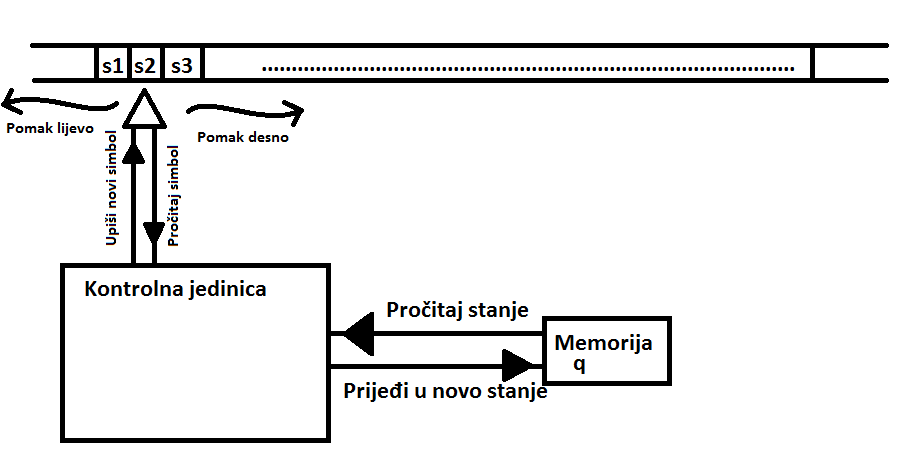
\includegraphics[height=200pt, width=400pt]{Turing.png}
\caption{Shematski prikaz Turingovog stroja}
\label{fig:Turing}
\end{figure} 
\begin{defn}
Neka su $f, g: \mathbb{N} \to \mathbb{R}^{+}$ dvije funkcije. Kažemo da je funkcija $g$ \textbf{asimptotska gornja međa} za funkciju $f$ ako postoje $c>0$ i $n_0 \in \mathbb{N}$ tako da za svaki $n \geq n_0$ vrijedi
\[f(n)\leq cg(n)\]
Činjenicu da je $g$ asimptotska međa od $f$ označavamo sa $f(n)=O(g(n)$. 
\end{defn}
Osnovne definicije (što je alfabet logike sudova, interpretacija, ispunjivost formule, konjunktivna, odnosno, disjunktivna normalna forma  i tako dalje) se mogu naći u \cite[str. ~12-25]{Vukovic}.\\
Više o Turingovom stroju te nekim pojmovima na koje se pozivamo u idućim rezultatima se mogu naći u:
\begin{itemize}
\item Turing prepoznatiljivost, Turing odlučivost \cite[str. ~141-142]{Sipser}
\item Vremenska složenost determinističkog Turingovog stroja se može naći u \cite[str. ~248]{Sipser}, a nedeterminističkog u \cite[str. ~255]{Sipser}
\item Klase vremenske složenosti:
 \begin{itemize}
 	\item $TIME(f(n))$ u \cite[str. ~251]{Sipser}
 	\item $\mathcal{P}$  u \cite[str. ~258]{Sipser}
 	\item Vezano uz klasu $\mathcal{NP}$ u \cite[str. ~265-267]{Sipser}
 \end{itemize} 
 	\item Polinomna reducibilnost u \cite[str. ~272]{Sipser}
 	\item $\mathcal{NP}$-potpunost u \cite[str. ~276]{Sipser}
\end{itemize}

Postavlja se prirodno pitanje kako izračunati složenost DNA računala. Odgovor je jednostavan: složenost DNA računala procijenjujemo brojem instrukcija koje DNA stroj izvrši, te s kardinalosti skupa $MulS(K)$. Zbog toga što kardinalnost skupa $MulS(K)$ može izrazito brzo rasti (samo jedna operacija \textit{Proširi(K)}, za pripadnu funkciju kratnosti $m$ multiskupa $MulS(K)$ vrijedi da je: $m_{nova}(x)=2\cdot m_{stara}(x)$, gdje je $m_{nova}(x)$ kratnost od $x$ nakon izvršenja operacije \textit{Proširi}, a $m_{stara}(x)$ kratnost od $x$ prije izvršenja te iste operacije) prostorna složenost nekog programa za DNA stroj obično doseže nadeksponencijalnu veličinu (vidjet ćemo u idućem potpoglavlju takav slučaj). \\
U sljedećem potpoglavlju ćemo procijeniti složenost jednog programa za DNA stroj.
\subsection{Problem Hamiltonovog puta}
\label{subsec:HPP}
\begin{defn}
\textbf{Konačan usmjereni graf} je uređeni par $G=(V,E)$ gdje je V proizvoljan konačan skup čije elemente nazivamo \textbf{vrhovi}, a $E\subseteq V \times V$ skup čije elemente nazivamo \textbf{bridovi}. Ako je $E=V\times	V$ kažemo da je usmjereni graf $G$ \textbf{potpuni graf}. Kažemo da je brid $e$ \textbf{petlja} ako vrijedi:
$(\exists x \in V) : e=(x,x)$.
\textbf{Šetnja u grafu} G je $2n+1$-torka $(v_0,e_0,v_1,e_1,...,v_{n-1},e_{n-1}, v_{n})$, pri čemu vrijedi:
\begin{itemize}
	\item $(\forall i \in \{0,...,n\}) \quad v_i \in V$
	\item $(\forall i \in \{0,...,n-1\}) \quad e_i \in E$
	\item $e_i=(v_i, v_{i+1}), \forall i \in \{0,...,n-1\}$
\end{itemize}
Kažemo da šetnja  $(v_0,e_0,v_1,e_1,...,v_{n-1},e_{n-1}, v_{n})$ \textbf{prolazi kroz vrh} $x \in V$ ako postoji $i \in \{0,...,n\}$ takav da je $x=v_i$, te da šetnja \textbf{počinje} s vrhom $v_0$ i \textbf{zavšrava} s vrhom $v_n$. Duljina šetnje se definira kao broj bridova koji se pojavljuju u njoj.\\
\textbf{Staza} u grafu je šetnja $(v_0,e_0,v_1,e_1,...,v_{n-1},e_{n-1}, v_{n})$ za koju vrijedi 
\[(\forall i,j \in \{0,...,n-1\})\, (i\neq j) \to e_i \neq e_j\] \textbf{Put} u grafu je šetnja $(v_0,e_0,v_1,e_1,...,v_{n-1},e_{n-1}, v_{n})$ za koju vrijedi:
\[(\forall i,j \in \{0,...,n\})\, (i\neq j) \to v_i \neq v_j\] \textbf{Hamiltonov put} je put koji prolazi kroz sve vrhove grafa G.
\end{defn}
\begin{nap}
Neusmjereni graf se definira analogno, ali se skup bridova definira kao:
\[E\subseteq \{\{x,y\} : x, y \in V\}\]
Također, radi jednostavnosti, pretpostavili smo da između dva vrha $x,y \in V$ može biti najviše dva usmjerena brida i u tom slučaju vrijedi: $(x,y) \in E$ i $(y,x) \in E$.  
\end{nap}
Problem Hamiltonovog puta glasi:\\
\begin{center}
\textit{Postoji li u proizvoljnom konačnom grafu $G=(V,E)$ za vrhove $x,y \in V$  Hamiltonov put koji počinje s $x$, a završava s $y$.}
\end{center}
U \cite[str. ~286-291]{Sipser} se može vidjeti da je problem Hamiltonovog puta $\mathcal{NP}$-potpun problem. U ovom poglavlju analiziramo \textit{Adlemanov algoritam} koji rješava problem u $\mathcal{O}(n \log (n))$ operacija. U kasnijim poglavljima ćemo obrazložiti reprezentaciju podataka pomoću DNA lanaca, za sada ćemo samo reći da su naši podaci reprezentirani lancima parne duljine $l$. Sada ćemo prezentirat Adlemanov algoriatam za traženje Hamiltonovog puta koji počinje s vrhom $v_{in}$, a završava s $v_{out}$ u usmjerenom označenom grafu $G=(V,E)$. Ali prije toga ćemo reći nešto o vezi bridova i vrhova. Ako su dani vrhovi $A$ i $B$ reprezentirani riječima $H$ i $J$, tada je brid $(A,B)$ reprezentiran riječju koja je nastala konkatenacijom (u smislu operacije nad riječima) biološkog sufiksa riječi $H$ i biološkog prefiksa riječi $J$. Kako bi mogli razlikovati koji brid povezuje koje vrhove, uviđamo da svaki vrh mora imati jedinstveni prefiks i sufiks, a ne samo jedinstven prikaz jednom riječju. 
    Nakon što smo objasnili vezu između bridova i vrhova moramo najprije "pripremiti" epruvetu za algoritam. \[K=V\cup E\]
    U početku je upravo $MulS(K)=K$.\\
    \indent Adlemanov algoritam:
    \begin{enumerate}
        \item Ulaz: Graf $G=(V,E)$, $|V|=n$, $v_1=v_{in}$ vrh iz kojeg krećemo, $v_n=v_{out}$ vrh u kojem završavamo, stavi vrhove i bridove u $K$
        \item $ \lceil 2n\log_{2}(n) \rceil$ puta primjeni operaciju \textit{Proširi(K)} tako da dobiješ barem $2^{2n\log_{2}(n)}=n^{2n}$ kopija svake riječi u $MulS(K)$
        \item Primjeni operaciju \textit{Konkatenacija(K)} da dobiješ šetnju u $G$, tako da duljina šetnje bude manja od $n$ - broj bridova u šetnji može biti manji ili jednak $n$
        \item Primjeni \textit{Odvoji\textunderscore Pref(K, $v_{in}$)}: izbacujemo one šetnje koje ne počinju vrhom $v_{in}$
        \item  \textit{Odvoji\textunderscore Suff(K, $v_{out}$)} : izbacujemo one šetnje koje ne završavaju s $v_{out}$
        \item Primjeni operaciju \textit{Izdvoji\textunderscore po \textunderscore duljini(K, $l\cdot n + l\cdot (n-1) $)} da iz $K (MulS(K))$ izbaciš sve one riječi koje u sebi ne sadrže točno $n$ vrhova i $n-1$ bridova (šetnje čija je duljina točno $n-1$)
        \item na $v_i$ primjeni operaciju \textit{Odvoji(K, $v_i$)} , $\forall{i} \in \{2,3,...,n-1\}$: iz $MulS(K)$ ukloni sve one šetnje u kojima se neki od vrhova ne pojavljuje
        \item \textit{Uoči(K)}: postoji li Hamiltonov put
    \end{enumerate}


Nama zapravo bridovi u ovom algoritmu, konstruirani na ovaj način, daju mogućnost povezivanja dva vrha koja su povezana nekim birdom (u smislu biokemije, bridovi igraju ulogu komplementarnog lanca koji  spajanjem s neka druga dva lanca daje strukturu dvostruke uzvojnice. \\
Brojimo korake algoritma:
\begin{itemize}
\item 2: $\lceil 2n \log _2 (n) \rceil$ koraka
\item  3-6: Po jedan korak svaka operacija
\item 7: $n-2$ koraka
\item 8: jedan korak
\end{itemize}
Ukupno: $\lceil 2n \log _2 (n) \rceil + n-2 + 5=\lceil 2n \log _2 (n) \rceil + n+3 = \mathcal{O}(n \log(n))$ operacija. No, rekli smo da se složenost DNA stroja mjeri i kardinalnošću skupa $MulS(K)$ koji u jednom trenutku sadrži i $n^{2n}$ elemenata. 
Još je preostalo dokazati da algoritam radi:
\begin{thm} Neka je G=(V,E) usmjeren označen graf, te $v_{in}$ i $v_{out}$ elementi iz V, tada Adlemanov algoritam odlučuje postoji li u usmjerenom grafu G=(V,E) Hamiltonov put od $v_{in}$ do $v_{out}$. \end{thm}

\begin{proof}
    \begin{itemize}
        \item $|V|=n$, $K=V\cup E$ gdje smatramo da je svakom vrhu dodijeljen jedinstven prefiks i sufiks. Neka je minimalni DNA lanac duljine $l$.
        \item Definiramo rekurzivno skupove $MulS(K_n)$ odakle ćemo zapravo izvući kako izgleda naš skup $MulS(K)$ nakon primjene operacije \textit{Proširi(K)} $\lceil 2n\log_2(n) \rceil$ puta
        \[K_0=K \to MulS(K_0)=K_0\]
        \[MulS(K_{n+1})=MulS(K_n) \cup MulS(K_n) , n \in \mathbb{N}\]
        Nakon ovog koraka, redefiniramo skup MulS(K)
        \[MulS(K)=MulS(K_{\lceil 2n\log_2(n) \rceil})\]
        Zapravo sada trebamo dokazati da je $2^{\lceil 2n\log_2(n) \rceil}$ dovoljan broj kopija skupa K za kreiranje svih šetnji u grafu:
        \[2^{\lceil 2n\log_2(n) \rceil} \geq 2^{ 2n\log_2(n) } = n^{2n}\]
        pa je dovoljno pokazati da je $n^{2n}$ dovoljan broj kopija skupa K od kojih možemo kreirati sve šetnje u grafu. Bez smanjenja općenitosti u tu svrhu možemo pretpostaviti da je G potpuno povezan usmjeren graf (dakle svaki brid je povezan sa svakim u oba smjera). Zašto? Jer ako G nije potpuno povezan onda ima manji broj šetnji od potpuno povezanog usmjerenog grafa. \\
        \noindent U tu svrhu definiramo skup $A^k$:
        \[A^k=\{(b_1,...,b_k): b_i \in V\}\]
        Uvidimo da smo u skupu $A^k$ dozvolili i petlje! Dakle može postojati brid $(v_i, v_i)$. Kada to ne bi dozvolili, na uređenu $k$-torku bi samo još stavili uvjet da je $b_i \neq b_{i+1}, \quad \forall i \in \{1,...,k-1\}$.
        Sada, jer između svaka 2 vrha ima točno 1 brid za svaki smjer koji povezuje te vrhove, vidimo da su sve šetnje duljine $k-1$ jedinstveno određene skupom $A^k$. Pa su sve šetnje do duljine $n-1$ (jer ćemo tako izabrati operaciju konkatenacije da kreira šetnje duljine ne duže od $n-1$) reprezentirane idućim skupom:
        \[\bigcup_{k=1}^n A^k\]
        Preostalo je dokazati da kardinalnost gornjeg skupa nije veća od $n^{2n}$. Kardinalnost skupa $A^k$ je lako odrediti. Naime za prvu komponentu uređene $k$-torke ima $n$ mogućnosti, za $2$ isto $n$, općenito za $i$-tu komponentu ima $n$ mogućnosti.
        \[|A^k|=n^k \to \bigg|\bigcup_{k=1}^n A^k\bigg|=\sum_{k=1}^n |A^k|=\sum_{k=1}^n n^k=\frac{n(n^n-1)}{n-1}\]
        \[\frac{n(n^n-1)}{n-1} \leq \frac{n\cdot n^n}{n-1} \leq n\cdot n^n =n^{n+1} \leq n^{2n}\]
        \item Primjenom operacije \textit{Konkatenacija(K)} dobili smo sve moguće šetnje u grafu $G$ (spremljene u $MulS(K)$)
        \item Operacijama \textit{Odvoji\textunderscore Pref(K, $v_{in}$)} i \textit{Odvoji\textunderscore Suff(K, $v_{out}$)} iz skupa $MulS(K)$ izbacujemo sve one šetnje koje ne počinju vrhovima $v_{in}$ i ne završavaju s $v_{out}$
        \item operacijom \textit{Izdvoji\textunderscore po\textunderscore duljini(K, $l\cdot n + l\cdot (n-1)$)} uklanjamo sve preostale bridove i one šetnje čija je duljina strogo manja od $n-1$.
        Sada su ostale šetnje duljine $n-1$, ali to još nisu putevi (a onda ni Hamiltonovi putevi). Kako ima $n$ vrhova, a šetnja je duljine $n-1$, to znači da je u šetnji točno $n$ vrhova kroz koje šetnja prolazi, ako se neki vrh ne nalazi u šetnji, to znači da se neki drugi vrh pojavljuje dva puta. A kako smo već uklonili one šetnje koje ne počinju s  $v_{in}$ i ne završavaju s $v_{out}$ jedino je preostalo ukloniti sve one šetnje koje ne sadrže neki $v_i \in V \backslash \{v_{in}, v_{out}\}$.
        \item Za svaki $x \in V \backslash \{v_{in}, v_{out}\}$ čini:
        \[Odvoji(K,x)\]
        \item Ovim su korakom zapravo u $MulS(K)$ ostali samo Hamiltonovi putevi koji počinju s  $v_{in}$ i završavaju s $v_{out}$, ako takvih ima, operacijom \textit{Uoči(K)} dobivamo rješenje.
    \end{itemize} 
\end{proof}
Ipak, zbog duljine trajanja biokemijskih reakcija teorijska istraživanja pokazuju da Adlemannov algoritam nije pogodan za riješavanje problema Hamiltonovog puta ako graf sadrži više od $70$ vrhova.\footnote{\cite{Lipton}}
\subsection{Liptonov teorem}
Označimo sa $SAT$ skup definiran na idući način:
\[SAT=\{F: F \textrm{ je ispunjiva formula logike sudova }\}\]
Formulacija \textit{problema SAT} glasi:\\
\begin{center}
Za danu formulu logike sudova F koja je u konjunktivnoj normalnoj formi odrediti\\ vrijedi li $F \in  SAT$.
\end{center}
Konjunktivnu normalnu formu koja u svakoj svojoj elementarnoj disjunkciji sadrži točno $k \in \mathbb{N} \backslash \{0\}$ literala nazivamo $k$-knf. Formulacija problema $k-SAT$ glasi:
\begin{center}
	Za proizvoljnu formulu $F$ koja je $k$-knf odrediti je li $F$ ispunjiva. 
\end{center} 
U \cite[str. ~276-283]{Sipser} se može vidjeti da je problem $SAT$ \textit{$\mathcal{NP}$-potpun} problem, kao i $3-SAT$.
Sljedeći teorem govori zapravo o tome da DNA računala, u pogledu vremenske složenosti, imaju bolja svojstva nego deterministički Turnigovi strojevi. No kako bi ga bolje shvatili objasnit ćemo skicu dokaza kroz jedan primjer.\\
Za svaki $n\in \N$ neka je $G_n=(V_n, E_n)$ graf opisan na sljedeći način:
\begin{itemize}
\item $V_n=\{x_1, \neg x_1, a_1, x_2, \neg x_2, a_2,..., x_n, \neg x_n, a_n, a_{n+1}\}$
\item  $E_n=\{(a_i, x_i), (a_i, \neg x_i), (x_i, a_{i+1}), (\neg x_i, a_{i+1}) | i \in \{1,...,n\}\}$
\end{itemize}
\begin{exa}
Graf $G_2$ se može vidjeti na slici \ref{fig:g2}.
\begin{figure}[!h]
\begin{center}
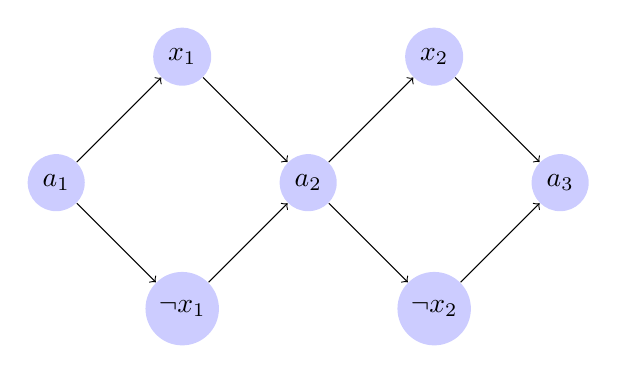
\begin{tikzpicture} [scale=.8,auto=left,every node/.style={circle,fill=blue!20}]
\node (A) at (0,2) {$a_1$};
\node (B) at (2,4) {$x_1$};
\node (C) at (2,0) {$\neg x_1$};
\node (D) at (4,2) {$a_2$};
\node (E) at (6,4) {$x_2$};
\node (F) at (6,0) {$\neg x_2$};
\node (G) at (8,2) {$a_3$};

\foreach \from/\to in {A/B,A/C,B/D,C/D,D/E,D/F,E/G,F/G}
\draw [->] (\from) -- (\to);
\end{tikzpicture}
\end{center}
\caption{Graf $G_2$}
\label{fig:g2}
\end{figure}
Sada svakom putu od $a_1$ do $a_3$ u $G_2$ odgovara jedan binarni niz duljine $2$. Tako na primjer put $a_1x_1a_2\neg x_2a_3$ možemo poistovjetiti sa nizom $10$. Formiranje puteva u grafu se inicijalizira na isti način kao što se to napravilo i u potpoglavlju \ref{subsec:HPP}. Operacije će se izvoditi samo na onim DNA nizovima koji predstavljaju vrhove u grafu $G_2$ ($G_n$) i to na idući način: $E(t,i,a)$ će označavati sve one DNA nizove (lance) epruvete $t$ čiji će ekvivalentni binarni nizovi na $i$-tom mjestu imati $a\in \{0,1\}$. Neka je sada
\begin{equation}
\label{eq:prim}
F \equiv (x_1 \vee x_2)  \wedge (\neg x_1 \vee \neg x_2)
\end{equation}

Konstruirat ćemo niz epruveta:
\begin{itemize}
\item $t_0$ sadrži sve binarne nizove duljine 2
\item $t_1 \leftarrow E(t_0,1,1)$, a $t_1'=t_0\backslash t_1$
\item $t_2 \leftarrow E(t_1', 2,1)$, 
\item $t_3=t_1 \cup t_2$ (sadržaj epruveta $t_1$ u $t_2$ smo ulili u epruvetu $t_3$)
\item $t_4 \leftarrow E(t_3, 1,0)$, a $t_4'=t_3\backslash t_4$
\item $t_5 \leftarrow E(t_4',2,0)$
\item $t_6=t_4 \cup t_5$
\end{itemize}
U konačnici nad $t_6$ počinimo operaciju \textit{Uoči} ($Detect$ u izvornom Adlemanovom modelu DNA računala). Kako bi bolje razumjeli sadržaj navedenih epruveta, pogledajmo sada tablicu
\begin{table}[!h]
\begin{center}
\begin{tabular}{|c|c|}
\hline 
Epruveta & Sadržaj \\ 
\hline 
$t_0$ & $00,01,10,11$ \\ 
\hline 
$t_1$ & $10,11$ \\ 
\hline 
$t_1'$ & $00,01$ \\ 
\hline 
$t_2$ & $01$ \\ 
\hline 
$t_3$ & $10,11,01$ \\ 
\hline 
$t_4$ & $01$ \\ 
\hline 
$t_4'$ & $10,11$ \\ 
\hline 
$t_5$ & $10$ \\ 
\hline 
$t_6$ & $10,01$ \\ 
\hline 
\end{tabular} 
\end{center}
\label{tab:primjer}
\caption{Biološko riješenje za ispunjivost formule \ref{eq:prim}}
\end{table}
\end{exa}
\begin{thm} (\textbf{Lipton})
Za svaku konjunktivnu normalnu formu $F$ u kojoj se pojavljuje $n$ propozicionalih varijabli i $m$ klauzula, u $\mathcal{O}(m)$ odvajanja (ekstrakcija) i $\mathcal{O}(m)$ spajanja te jednim uočavanjem možemo odlučiti vrijedi li $F \in SAT$.
\end{thm}
\begin{proof}
Neka je:
\begin{equation}
\label{eq:knf}
F\equiv \bigwedge_{i=1}^m C_i
\end{equation} 
Gdje je $C_j$ klauzula koja se sadrži od fiksnog broja literala. Konstruirat ćemo epruvete $t_k$.
$t_0,...,t_m$ su konstruirane tako da $t_k$ sadrži $n$-bitne brojeve $x=x_1...x_n$ za koje vrijedi $C_1(x)=C_2(x)=...=C_k(x)=1$, gdje je $C_i(x)$ vrijednost klauzule $C_i$ za vrijednost literala klauzule $C_i$ postavljenih na vrijednost bitova od $x$.
\[t_0=\{x_1...x_n |x_i \in \{0,...,1\}\}\]
Neka je sada $C_{k}$ sljedeća klauzula:
\[v_1^{(k)} \vee ... \vee v_l^{(k)}\]
Gdje je $v_i^{(k)}$ literal. \\
\noindent\rule{8cm}{0.4pt}\\
$t_0=\{x_1...x_n |x_i \in \{0,...,1\}\}$\\
$\forall k \in \{0,...,m-1\}$	
\begin{itemize}
\item $t_{k+1}=\emptyset$
\item $\forall i \in \{1,...,l\}$ (Prolazimo po literalima klauzule)
\begin{itemize}
\item $ \forall	j \in \{1,...,n\}$ (Prolazimo po vrhovima grafa $G_n$)
	\begin{itemize}
		\item Ako $v_i ^{(k)}==x_j$
		\begin{itemize}
			\item  $t_{k+1} \leftarrow t_{k+1} \cup E(t_{k}\backslash t_{k+1},j,1)$
		\end{itemize}
		\item Ako $v_i^{(k)}==\neg x_j$
		\begin{itemize}
			\item $t_{k+1} \leftarrow t_{k+1} \cup E(t_{k} \backslash t_{k+1},j,0)$
		\end{itemize}
	\end{itemize}
\end{itemize}
\end{itemize}
$Detect(t_m)$\\
\noindent\rule{8cm}{0.4pt}\\
Još je ostalo dokazati da na ovaj način konstruirane epruvete $t_k$  sadržavaju sve $n$-bitne brojeve $x$ koji zadovoljavaju: \begin{equation}
\label{eq:svojstvo}
C_1(x)=...=C_k(x)=1
\end{equation}
Dokaz ide indukcijom po $k$. Pretpostavimo da tvrdnja vrijedi za sve $n \in \N \backslash \{0\}$ takve da $n \leq k$. Pogledajmo vrijedi li tvrdnja za $k+1$. Vidimo da je $t_{k+1}$ konstruirana iz $t_k$ za koju je zadovoljeno \ref{eq:svojstvo}. Ako se sada bilo koji $v_i ^{(k+1)}$ podudara s nekim $x_j$ za neki $j$, onda će se za $t_{k+1}$ napraviti isti korak kao i za $t_k$, a to je:
\[t_{k+1} \leftarrow t_{k+1} \cup E(t_{k}\backslash t_{k+1},j,1)\]
Pa će one sadržavati iste one brojeve $x$ koji na $j$-tom mjestu imaju $1$, a za njih je zadovoljeno svojstvo \ref{eq:svojstvo} (nalazili su se u $t_k$). Analogno se razmatra slučaj $v_i ^{(k+1)}==\neg x_j$. Ako se pak dogodi slučaj da za svaki $j$ $t_k$ ne sadrži niti jedan $x$ koji na mjestu $j$ sadrži: 
\begin{itemize}
\item $1$ ako zadovoljen uvjet $v_i^{(k+1)}==x_j$
\item $0$ ako zadovoljen uvjet $v_i^{(k+1)}==\neg x_j$
\end{itemize} 
Onda $t_{k+1}$ ostaje prazan za sve iteracije ukoliko se to dogodilo za sve $v_i^{(k+1)}$, pa će vrijediti da ne postoji $x$ za kojeg bi vrijedilo $C_{k+1}(x)=1$, time će se pak dobiti da formula zapravo nije ispunjiva jer će i $t_{m}$ onda ostati prazan. Slučaj $k>m$ nije potrebno razmatrati (jednostavno se postavi da je $t_k=\emptyset$ u tom slučaju). \\
Duljina svake klauzule $C_i$ je fiksna (iznosi $l$). Već unaprijed smo pripremili reprezentaciju vrhova i svih binarnih nizova duljine $n$ u $t_0$ pa je i $n$ već fiksan na ulazu u naš algoritam (važno je napomenuti da za ulaz Lipton nije razmatrao broj koraka potreban za inicijalnu epruvetu, već je podrazumijevao da je ona pripremljena). Ukupno se "vrte" tri petlje, a ključni koraci su zapravo unutar uvjeta koji se nalaze u najdubljoj petlji. Kada je to sve uzeto u obzir imamo da je:
\begin{itemize}
	\item $n \cdot l \cdot m$ odvajanja
	\item Epruveta $t_{k+1}$ je na početku svakog koraka prazna, pa se unija (spajanje dviju epruveta) za $i=1 \wedge j=1$ ne broji pa je to $m \cdot l \cdot n - n=mln-n=n(ml-1)$ spajanja
\end{itemize}
Na kraju imamo samo jednu detekciju. Iz čega slijedi tvrdnja teorema. Ukupan broj koraka je $\mathcal{O}(m)$   
\end{proof}
"Gornji teorem implicira da se biološko izračunavanje može koristiti kako bi se riješili svi problemu u klasi $\mathcal{NP}$, ali to ne znači da se sve instance klase $\mathcal{NP}$ mogu riješiti na zadovoljiv način."\footnote{\cite[str. ~407]{CNTYan}} Time se hoće reći da se većina takvih problema na DNA računalu rješavaju grubom silom. U kasnijim razmatranjima ćemo vidjeti da to za DNA računala nije uvijek pogodno - naime biokemijske reakcije se usporavaju čim epruveta sadrži više (dužih) DNA lanaca, te čim ti lanci u sebi imaju više veza između citozina i gvanina.   
S pogleda odlučivosti jezika, odnosno izračunljivosti ipak nemamo takav rezultat, odnosno postoji slutnja koja kaže:
\begin{conj} \cite{CNTYan} (Kvantna i biološka slutnja) Problem je odlučiv na DNA računalu ili kvantnom računalu ako i samo ako je Turing-odlučiv.
Nadalje, proizvoljna funkcija $f: S \subset \N^k \to \N$ je DNA-izračunljiva, odnosno kvantno izračunljiva ako i samo ako je Turing-izračunljiva.
\end{conj}
Lipton je također pokazao da se pomoću DNA računala može generalizirati slučaj - odlučivanje ispunjivosti generalnih formula logike sudova (one koje koriste veznike $\neg, \vee, \wedge$) koje nisu nužno knf. O tome se više može pročitati u \cite{Lipton}. 
\section{Prednosti i mane DNA računala}
U ovom seminaru smo se upoznali s nekim temeljnim prednostima DNA računala (na primjer rješavanje problema Hamiltonova puta, Liptonov teorem), no nismo ništa rekli koje su mane DNA računala. Prije nego ih navedemo, navedimo još neke prednosti koje nisu spomenute u ovom radu:\\
DNA računala imaju izrazito veliki kapacitet memorije i gustoću  zbog koje se stvari mogu lakše izračunavati. Na primjer u jedan gram DNA lanaca se može pohraniti $5.5$ petabita ($=5.5\cdot 10^{15}$ bita) što je otprilike $700$ terabajta $= 700 \cdot 10^{12}$ bajta, a o tome se može pročitati u \cite{Church}. Zbog tolike gustoće u memoriji i masivne paralelnosti DNA računala (jedna operacija se obavlja nad skupom riječi, a ne na samo jednoj riječi (broj procesora varira - to je kao da broj procesora konstantno varira ovisno o broju podataka u programu)) mnogi problemi se riješavaju upravo primjenom tehnike grube sile. S druge strane, kada bi se DNA računalo i u stvarnosti konstruiralo, biokemijski procesi se ne odvijaju bez greške. Rađena su istraživanja kako utjecati na te greške, a među njima je jedno napisao i Lipton što se može vidjeti u \cite{DNAerr}. Zbog toga što se biokemijske reakcije ne izvršavaju trenutno već za njih treba vremena (slamanje kovalentnih veza pa opet sastavljanje istih) i pripreme, one postaju spore za izvršavanje. Štoviše, njihovo izvršavanje nad DNA lancima postaje sporije čim su ti DNA lanci duži te čim je više DNA lanaca u epruveti, ali i biokemijski gledano - što je više parova $C-G$ između dva komplementarna DNA lanca, te lance je teže razdvojiti zbog trostrukih kovalentnih veza. Unatoč ovome, ne smijemo zaboraviti da područja genetike i medicine napreduju te da će se možda doći do otkrića kako te operacije ubrzati.
\newpage
\nocite{*}
\bibliographystyle{abbrv}
\bibliography{literatura}
\end{spacing}
\end{document}